% Graphic for TeX using PGF
% Title: /mnt/64BB-4184/Filing/Education/Lund/Courses/NumericsSeminar/numerics-seminar-VT23/Figures/Diagram_001.dia
% Creator: Dia v0.97+git
% CreationDate: Mon Apr 17 10:23:22 2023
% For: theo
% \usepackage{tikz}
% The following commands are not supported in PSTricks at present
% We define them conditionally, so when they are implemented,
% this pgf file will use them.
\ifx\du\undefined
  \newlength{\du}
\fi
\setlength{\du}{15\unitlength}
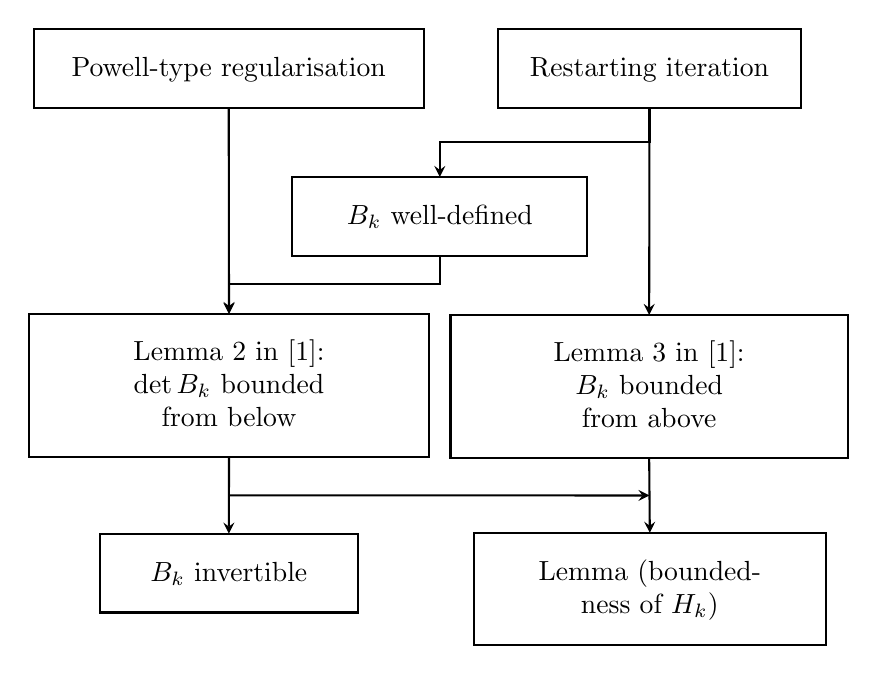
\begin{tikzpicture}[even odd rule]
\pgftransformxscale{1.000000}
\pgftransformyscale{-1.000000}
\definecolor{dialinecolor}{rgb}{0.000000, 0.000000, 0.000000}
\pgfsetstrokecolor{dialinecolor}
\pgfsetstrokeopacity{1.000000}
\definecolor{diafillcolor}{rgb}{1.000000, 1.000000, 1.000000}
\pgfsetfillcolor{diafillcolor}
\pgfsetfillopacity{1.000000}
\pgfsetlinewidth{0.050000\du}
\pgfsetdash{}{0pt}
\pgfsetmiterjoin
{\pgfsetcornersarced{\pgfpoint{0.000000\du}{0.000000\du}}\definecolor{diafillcolor}{rgb}{1.000000, 1.000000, 1.000000}
\pgfsetfillcolor{diafillcolor}
\pgfsetfillopacity{1.000000}
\fill (39.300400\du,9.156810\du)--(39.300400\du,12.606810\du)--(48.872900\du,12.606810\du)--(48.872900\du,9.156810\du)--cycle;
}{\pgfsetcornersarced{\pgfpoint{0.000000\du}{0.000000\du}}\definecolor{dialinecolor}{rgb}{0.000000, 0.000000, 0.000000}
\pgfsetstrokecolor{dialinecolor}
\pgfsetstrokeopacity{1.000000}
\draw (39.300400\du,9.156810\du)--(39.300400\du,12.606810\du)--(48.872900\du,12.606810\du)--(48.872900\du,9.156810\du)--cycle;
}% setfont left to latex
\definecolor{dialinecolor}{rgb}{0.000000, 0.000000, 0.000000}
\pgfsetstrokecolor{dialinecolor}
\pgfsetstrokeopacity{1.000000}
\definecolor{diafillcolor}{rgb}{0.000000, 0.000000, 0.000000}
\pgfsetfillcolor{diafillcolor}
\pgfsetfillopacity{1.000000}
\node[anchor=base,inner sep=0pt, outer sep=0pt,color=dialinecolor] at (44.086650\du,10.275873\du){Lemma 3 in \ensuremath{[}1\ensuremath{]}:};
% setfont left to latex
\definecolor{dialinecolor}{rgb}{0.000000, 0.000000, 0.000000}
\pgfsetstrokecolor{dialinecolor}
\pgfsetstrokeopacity{1.000000}
\definecolor{diafillcolor}{rgb}{0.000000, 0.000000, 0.000000}
\pgfsetfillcolor{diafillcolor}
\pgfsetfillopacity{1.000000}
\node[anchor=base,inner sep=0pt, outer sep=0pt,color=dialinecolor] at (44.086650\du,11.075873\du){$\norm{B_k}$ bounded};
% setfont left to latex
\definecolor{dialinecolor}{rgb}{0.000000, 0.000000, 0.000000}
\pgfsetstrokecolor{dialinecolor}
\pgfsetstrokeopacity{1.000000}
\definecolor{diafillcolor}{rgb}{0.000000, 0.000000, 0.000000}
\pgfsetfillcolor{diafillcolor}
\pgfsetfillopacity{1.000000}
\node[anchor=base,inner sep=0pt, outer sep=0pt,color=dialinecolor] at (44.086650\du,11.875873\du){from above};
\pgfsetlinewidth{0.050000\du}
\pgfsetdash{}{0pt}
\pgfsetmiterjoin
{\pgfsetcornersarced{\pgfpoint{0.000000\du}{0.000000\du}}\definecolor{diafillcolor}{rgb}{1.000000, 1.000000, 1.000000}
\pgfsetfillcolor{diafillcolor}
\pgfsetfillopacity{1.000000}
\fill (29.140300\du,9.135170\du)--(29.140300\du,12.585170\du)--(38.790300\du,12.585170\du)--(38.790300\du,9.135170\du)--cycle;
}{\pgfsetcornersarced{\pgfpoint{0.000000\du}{0.000000\du}}\definecolor{dialinecolor}{rgb}{0.000000, 0.000000, 0.000000}
\pgfsetstrokecolor{dialinecolor}
\pgfsetstrokeopacity{1.000000}
\draw (29.140300\du,9.135170\du)--(29.140300\du,12.585170\du)--(38.790300\du,12.585170\du)--(38.790300\du,9.135170\du)--cycle;
}% setfont left to latex
\definecolor{dialinecolor}{rgb}{0.000000, 0.000000, 0.000000}
\pgfsetstrokecolor{dialinecolor}
\pgfsetstrokeopacity{1.000000}
\definecolor{diafillcolor}{rgb}{0.000000, 0.000000, 0.000000}
\pgfsetfillcolor{diafillcolor}
\pgfsetfillopacity{1.000000}
\node[anchor=base,inner sep=0pt, outer sep=0pt,color=dialinecolor] at (33.965300\du,10.254233\du){Lemma 2 in \ensuremath{[}1\ensuremath{]}:};
% setfont left to latex
\definecolor{dialinecolor}{rgb}{0.000000, 0.000000, 0.000000}
\pgfsetstrokecolor{dialinecolor}
\pgfsetstrokeopacity{1.000000}
\definecolor{diafillcolor}{rgb}{0.000000, 0.000000, 0.000000}
\pgfsetfillcolor{diafillcolor}
\pgfsetfillopacity{1.000000}
\node[anchor=base,inner sep=0pt, outer sep=0pt,color=dialinecolor] at (33.965300\du,11.054233\du){$\abs{\det B_k}$ bounded};
% setfont left to latex
\definecolor{dialinecolor}{rgb}{0.000000, 0.000000, 0.000000}
\pgfsetstrokecolor{dialinecolor}
\pgfsetstrokeopacity{1.000000}
\definecolor{diafillcolor}{rgb}{0.000000, 0.000000, 0.000000}
\pgfsetfillcolor{diafillcolor}
\pgfsetfillopacity{1.000000}
\node[anchor=base,inner sep=0pt, outer sep=0pt,color=dialinecolor] at (33.965300\du,11.854233\du){from below };
\pgfsetlinewidth{0.050000\du}
\pgfsetdash{}{0pt}
\pgfsetmiterjoin
{\pgfsetcornersarced{\pgfpoint{0.000000\du}{0.000000\du}}\definecolor{diafillcolor}{rgb}{1.000000, 1.000000, 1.000000}
\pgfsetfillcolor{diafillcolor}
\pgfsetfillopacity{1.000000}
\fill (30.849200\du,14.424300\du)--(30.849200\du,16.324300\du)--(37.074200\du,16.324300\du)--(37.074200\du,14.424300\du)--cycle;
}{\pgfsetcornersarced{\pgfpoint{0.000000\du}{0.000000\du}}\definecolor{dialinecolor}{rgb}{0.000000, 0.000000, 0.000000}
\pgfsetstrokecolor{dialinecolor}
\pgfsetstrokeopacity{1.000000}
\draw (30.849200\du,14.424300\du)--(30.849200\du,16.324300\du)--(37.074200\du,16.324300\du)--(37.074200\du,14.424300\du)--cycle;
}% setfont left to latex
\definecolor{dialinecolor}{rgb}{0.000000, 0.000000, 0.000000}
\pgfsetstrokecolor{dialinecolor}
\pgfsetstrokeopacity{1.000000}
\definecolor{diafillcolor}{rgb}{0.000000, 0.000000, 0.000000}
\pgfsetfillcolor{diafillcolor}
\pgfsetfillopacity{1.000000}
\node[anchor=base,inner sep=0pt, outer sep=0pt,color=dialinecolor] at (33.961700\du,15.568363\du){$B_k$ invertible};
\pgfsetlinewidth{0.050000\du}
\pgfsetdash{}{0pt}
\pgfsetmiterjoin
{\pgfsetcornersarced{\pgfpoint{0.000000\du}{0.000000\du}}\definecolor{diafillcolor}{rgb}{1.000000, 1.000000, 1.000000}
\pgfsetfillcolor{diafillcolor}
\pgfsetfillopacity{1.000000}
\fill (35.487500\du,5.833200\du)--(35.487500\du,7.733200\du)--(42.600000\du,7.733200\du)--(42.600000\du,5.833200\du)--cycle;
}{\pgfsetcornersarced{\pgfpoint{0.000000\du}{0.000000\du}}\definecolor{dialinecolor}{rgb}{0.000000, 0.000000, 0.000000}
\pgfsetstrokecolor{dialinecolor}
\pgfsetstrokeopacity{1.000000}
\draw (35.487500\du,5.833200\du)--(35.487500\du,7.733200\du)--(42.600000\du,7.733200\du)--(42.600000\du,5.833200\du)--cycle;
}% setfont left to latex
\definecolor{dialinecolor}{rgb}{0.000000, 0.000000, 0.000000}
\pgfsetstrokecolor{dialinecolor}
\pgfsetstrokeopacity{1.000000}
\definecolor{diafillcolor}{rgb}{0.000000, 0.000000, 0.000000}
\pgfsetfillcolor{diafillcolor}
\pgfsetfillopacity{1.000000}
\node[anchor=base,inner sep=0pt, outer sep=0pt,color=dialinecolor] at (39.043750\du,6.977263\du){$B_k$ well-defined};
\pgfsetlinewidth{0.050000\du}
\pgfsetdash{}{0pt}
\pgfsetmiterjoin
{\pgfsetcornersarced{\pgfpoint{0.000000\du}{0.000000\du}}\definecolor{diafillcolor}{rgb}{1.000000, 1.000000, 1.000000}
\pgfsetfillcolor{diafillcolor}
\pgfsetfillopacity{1.000000}
\fill (39.863600\du,14.404400\du)--(39.863600\du,17.104400\du)--(48.341100\du,17.104400\du)--(48.341100\du,14.404400\du)--cycle;
}{\pgfsetcornersarced{\pgfpoint{0.000000\du}{0.000000\du}}\definecolor{dialinecolor}{rgb}{0.000000, 0.000000, 0.000000}
\pgfsetstrokecolor{dialinecolor}
\pgfsetstrokeopacity{1.000000}
\draw (39.863600\du,14.404400\du)--(39.863600\du,17.104400\du)--(48.341100\du,17.104400\du)--(48.341100\du,14.404400\du)--cycle;
}% setfont left to latex
\definecolor{dialinecolor}{rgb}{0.000000, 0.000000, 0.000000}
\pgfsetstrokecolor{dialinecolor}
\pgfsetstrokeopacity{1.000000}
\definecolor{diafillcolor}{rgb}{0.000000, 0.000000, 0.000000}
\pgfsetfillcolor{diafillcolor}
\pgfsetfillopacity{1.000000}
\node[anchor=base,inner sep=0pt, outer sep=0pt,color=dialinecolor] at (44.102350\du,15.548463\du){Lemma (bounded-};
% setfont left to latex
\definecolor{dialinecolor}{rgb}{0.000000, 0.000000, 0.000000}
\pgfsetstrokecolor{dialinecolor}
\pgfsetstrokeopacity{1.000000}
\definecolor{diafillcolor}{rgb}{0.000000, 0.000000, 0.000000}
\pgfsetfillcolor{diafillcolor}
\pgfsetfillopacity{1.000000}
\node[anchor=base,inner sep=0pt, outer sep=0pt,color=dialinecolor] at (44.102350\du,16.348463\du){ness of $\norm{H_k}$)};
\pgfsetlinewidth{0.050000\du}
\pgfsetdash{}{0pt}
\pgfsetmiterjoin
{\pgfsetcornersarced{\pgfpoint{0.000000\du}{0.000000\du}}\definecolor{diafillcolor}{rgb}{1.000000, 1.000000, 1.000000}
\pgfsetfillcolor{diafillcolor}
\pgfsetfillopacity{1.000000}
\fill (40.452400\du,2.261550\du)--(40.452400\du,4.161550\du)--(47.737400\du,4.161550\du)--(47.737400\du,2.261550\du)--cycle;
}{\pgfsetcornersarced{\pgfpoint{0.000000\du}{0.000000\du}}\definecolor{dialinecolor}{rgb}{0.000000, 0.000000, 0.000000}
\pgfsetstrokecolor{dialinecolor}
\pgfsetstrokeopacity{1.000000}
\draw (40.452400\du,2.261550\du)--(40.452400\du,4.161550\du)--(47.737400\du,4.161550\du)--(47.737400\du,2.261550\du)--cycle;
}% setfont left to latex
\definecolor{dialinecolor}{rgb}{0.000000, 0.000000, 0.000000}
\pgfsetstrokecolor{dialinecolor}
\pgfsetstrokeopacity{1.000000}
\definecolor{diafillcolor}{rgb}{0.000000, 0.000000, 0.000000}
\pgfsetfillcolor{diafillcolor}
\pgfsetfillopacity{1.000000}
\node[anchor=base,inner sep=0pt, outer sep=0pt,color=dialinecolor] at (44.094900\du,3.405613\du){Restarting iteration};
\pgfsetlinewidth{0.050000\du}
\pgfsetdash{}{0pt}
\pgfsetmiterjoin
{\pgfsetcornersarced{\pgfpoint{0.000000\du}{0.000000\du}}\definecolor{diafillcolor}{rgb}{1.000000, 1.000000, 1.000000}
\pgfsetfillcolor{diafillcolor}
\pgfsetfillopacity{1.000000}
\fill (29.260500\du,2.279000\du)--(29.260500\du,4.179000\du)--(38.655500\du,4.179000\du)--(38.655500\du,2.279000\du)--cycle;
}{\pgfsetcornersarced{\pgfpoint{0.000000\du}{0.000000\du}}\definecolor{dialinecolor}{rgb}{0.000000, 0.000000, 0.000000}
\pgfsetstrokecolor{dialinecolor}
\pgfsetstrokeopacity{1.000000}
\draw (29.260500\du,2.279000\du)--(29.260500\du,4.179000\du)--(38.655500\du,4.179000\du)--(38.655500\du,2.279000\du)--cycle;
}% setfont left to latex
\definecolor{dialinecolor}{rgb}{0.000000, 0.000000, 0.000000}
\pgfsetstrokecolor{dialinecolor}
\pgfsetstrokeopacity{1.000000}
\definecolor{diafillcolor}{rgb}{0.000000, 0.000000, 0.000000}
\pgfsetfillcolor{diafillcolor}
\pgfsetfillopacity{1.000000}
\node[anchor=base,inner sep=0pt, outer sep=0pt,color=dialinecolor] at (33.958000\du,3.423062\du){Powell-type regularisation};
\pgfsetlinewidth{0.050000\du}
\pgfsetdash{}{0pt}
\pgfsetbuttcap
{
\definecolor{diafillcolor}{rgb}{0.000000, 0.000000, 0.000000}
\pgfsetfillcolor{diafillcolor}
\pgfsetfillopacity{1.000000}
% was here!!!
\pgfsetarrowsend{stealth}
\definecolor{dialinecolor}{rgb}{0.000000, 0.000000, 0.000000}
\pgfsetstrokecolor{dialinecolor}
\pgfsetstrokeopacity{1.000000}
\draw (33.958000\du,4.179000\du)--(33.965300\du,9.135170\du);
}
\pgfsetlinewidth{0.050000\du}
\pgfsetdash{}{0pt}
\pgfsetmiterjoin
\pgfsetbuttcap
{
\definecolor{diafillcolor}{rgb}{0.000000, 0.000000, 0.000000}
\pgfsetfillcolor{diafillcolor}
\pgfsetfillopacity{1.000000}
% was here!!!
\pgfsetarrowsend{stealth}
{\pgfsetcornersarced{\pgfpoint{0.000000\du}{0.000000\du}}\definecolor{dialinecolor}{rgb}{0.000000, 0.000000, 0.000000}
\pgfsetstrokecolor{dialinecolor}
\pgfsetstrokeopacity{1.000000}
\draw (44.094900\du,4.161550\du)--(44.094900\du,4.997375\du)--(39.043750\du,4.997375\du)--(39.043750\du,5.833200\du);
}}
\pgfsetlinewidth{0.050000\du}
\pgfsetdash{}{0pt}
\pgfsetbuttcap
{
\definecolor{diafillcolor}{rgb}{0.000000, 0.000000, 0.000000}
\pgfsetfillcolor{diafillcolor}
\pgfsetfillopacity{1.000000}
% was here!!!
\pgfsetarrowsend{stealth}
\definecolor{dialinecolor}{rgb}{0.000000, 0.000000, 0.000000}
\pgfsetstrokecolor{dialinecolor}
\pgfsetstrokeopacity{1.000000}
\draw (44.094900\du,4.161550\du)--(44.086700\du,9.156810\du);
}
\pgfsetlinewidth{0.050000\du}
\pgfsetdash{}{0pt}
\pgfsetmiterjoin
\pgfsetbuttcap
{
\definecolor{diafillcolor}{rgb}{0.000000, 0.000000, 0.000000}
\pgfsetfillcolor{diafillcolor}
\pgfsetfillopacity{1.000000}
% was here!!!
\pgfsetarrowsend{stealth}
{\pgfsetcornersarced{\pgfpoint{0.000000\du}{0.000000\du}}\definecolor{dialinecolor}{rgb}{0.000000, 0.000000, 0.000000}
\pgfsetstrokecolor{dialinecolor}
\pgfsetstrokeopacity{1.000000}
\draw (39.043750\du,7.733200\du)--(39.043750\du,8.421471\du)--(33.965300\du,8.421471\du)--(33.965300\du,9.109743\du);
}}
\pgfsetlinewidth{0.050000\du}
\pgfsetdash{}{0pt}
\pgfsetbuttcap
{
\definecolor{diafillcolor}{rgb}{0.000000, 0.000000, 0.000000}
\pgfsetfillcolor{diafillcolor}
\pgfsetfillopacity{1.000000}
% was here!!!
\pgfsetarrowsend{stealth}
\definecolor{dialinecolor}{rgb}{0.000000, 0.000000, 0.000000}
\pgfsetstrokecolor{dialinecolor}
\pgfsetstrokeopacity{1.000000}
\draw (33.965300\du,12.585200\du)--(33.961700\du,14.424300\du);
}
\pgfsetlinewidth{0.050000\du}
\pgfsetdash{}{0pt}
\pgfsetbuttcap
{
\definecolor{diafillcolor}{rgb}{0.000000, 0.000000, 0.000000}
\pgfsetfillcolor{diafillcolor}
\pgfsetfillopacity{1.000000}
% was here!!!
\pgfsetarrowsend{stealth}
\definecolor{dialinecolor}{rgb}{0.000000, 0.000000, 0.000000}
\pgfsetstrokecolor{dialinecolor}
\pgfsetstrokeopacity{1.000000}
\draw (33.963500\du,13.504700\du)--(44.094500\du,13.505600\du);
}
\pgfsetlinewidth{0.050000\du}
\pgfsetdash{}{0pt}
\pgfsetbuttcap
{
\definecolor{diafillcolor}{rgb}{0.000000, 0.000000, 0.000000}
\pgfsetfillcolor{diafillcolor}
\pgfsetfillopacity{1.000000}
% was here!!!
\pgfsetarrowsend{stealth}
\definecolor{dialinecolor}{rgb}{0.000000, 0.000000, 0.000000}
\pgfsetstrokecolor{dialinecolor}
\pgfsetstrokeopacity{1.000000}
\draw (44.086700\du,12.606800\du)--(44.102400\du,14.404400\du);
}
\end{tikzpicture}
